\documentclass[a4paper,12pt]{article} % тип документа

% Поля страниц
\usepackage[left=2.5cm,right=2.5cm,top=1.5cm,bottom=2cm,bindingoffset=0cm]{geometry}
    
% Отступ после заголовка
\usepackage{indentfirst}

% Картинки
\usepackage{graphicx}
\graphicspath{{images/}}
\usepackage{placeins}

% Таблицы
\usepackage{booktabs}
\usepackage{floatrow}

% Русский язык
\usepackage{cmap}  % поиск в PDF
\usepackage{mathtext}  % русские буквы в формулах
\usepackage[T2A]{fontenc}  % кодировка
\usepackage[utf8]{inputenc}  % кодировка исходного текста
\usepackage[english,russian]{babel}  % локализация и переносы

% Математика
\usepackage{amsmath}

% Ссылки TODO
% \usepackage[unicode=true]{hyperref}
% \usepackage[T1]{fontenc}

\begin{document}

\begin{center}   
	\large{Лабораторная работа № 2.1.5\\\textbf{Исследование термических эффектов при упругих деформациях}}\\
\end{center}

\section{Аннотация}

\noindent\textbf{Цель работы:}
экспериментально получить закон упругой деформации резины при постоянной температуре в зависимости от растягивающей силы; измерить нагрев резины при адиабатическом растяжении и определить её теплоёмкость.
	
\smallskip
\noindent\textbf{В работе используются:}
образец резины (тонкая полоса), закреплённый в теплоизолированном кожухе; набор грузов; термопара; цифровой осциллограф или микровольтметр.

\section{Теоретические сведения}

\subsection*{Общие сведения}
Работа, совершаемая образцом, складывается из работы по растяжению и работы против внешнего давления:
\begin{equation}
\delta A = -fdl + PdV,
\end{equation}
где $P$ - атмосферное давление.

Так как коэффициент Пуассона резины близок к 1/2, то относительное изменение объема значительно меньше изменения длины:
\begin{equation}
dU \approx TdS + fdl,
\end{equation}
где $TdS = \delta Q$ - переданная образцу теплота, выраженная через энтропию $S$.

Центральная формула, описывающая упругие свойства вещества:
\begin{equation}
f = (\frac{\partial U}{\partial l})_T - T(\frac{\partial S}{\partial l})_T.
\end{equation}
Эта формула показывает, что упругие свойства вещества определяются не
только зависимостью его внутренней энергии от деформации, но и изменением его энтропии. В большинстве твёрдых тел доминирующим является первое слагаемое, тогда как в резине (а также в газах) преобладает второе

\subsection*{Термодинамика резины}

Ввиду малого изменения обьема, счатаем резину идеальной:
\begin{equation}
U = U(T)
\end{equation}

\subsubsection*{\centering Изотермическое растяжение}
\begin{equation}
f = -T(\frac{\partial S}{\partial l})_T = T(\frac{\partial f}{\partial T})_l
\end{equation}

Отсюда однозначно выполнено:
\begin{equation}
f(T, l) = \frac{T}{T_0}\tilde{f}({\frac{l}{l_0}}).
\end{equation}
где $\tilde{f}({\frac{l}{l_0}})$ - некоторая функция, зависящая только от растяжения образца. Откуда модуль Юнга резины должен быть прямо пропорционален абсолютной температуре.

\subsubsection*{\centering Адиабатическое растяжение}

\begin{equation}
dU= fdl = C_ldT,
\end{equation}
где $C_l$ - теплоёмкость резины при постоянном удлинении.

Считая изменение температуры малым:
\begin{equation}
\Delta T = \frac{A_{внеш}}{C_l}
\end{equation}

\subsection*{Закон растяжения резины}

Для модели иделаьной полимерной сетки:
\begin{equation}
\Delta S(\lambda) \approx -const \cdot (\lambda^2+\frac{2}{\lambda}), \ \lambda = \frac{l}{l_0}
\end{equation}

\begin{equation}
f(T, \lambda) = s_0E\cdot \frac{1}{3}(\lambda-\frac{1}{\lambda^2})
\end{equation}
где $s_0$ - площадь поперечного сечения недеформированного образца, $E$ = $E_0 \frac{T}{T_0}$ - модуль Юнга резины, зависящий от температуры

\section{Используемое оборудование}

Схема установки приведена на рис.~\ref{ris:setup}. Исследуемый образец резины 1 расположен внутри кожуха из оргстекла 2 и закреплен по торцам в двух зажимах 3, 11. Верхний зажим неподвижен, а нижний может перемещаться вдоль двух верти- кальных направляющих 4. Положение нижнего зажима определяется с помощью линейки 10, размещенной позади него. К подвижному зажиму 3 подвешена легкая платформа 5, расположенная снаружи кожуха. Резина растягивается грузом Р, помещаемым на платформу. Растяжение образца может быть ограничено положением упора 7, фиксируемого винтами 6, 9 на стойках 8.	
\begin{figure}[H]
    \center{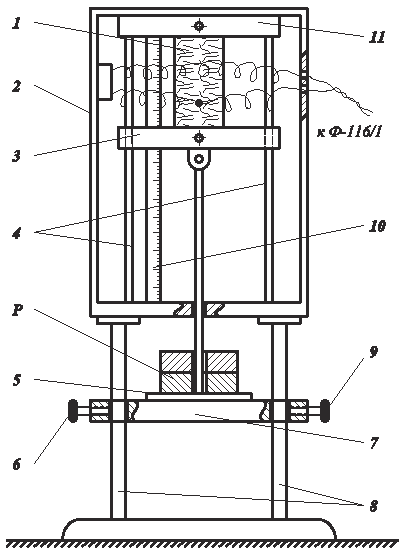
\includegraphics[scale=1]{установка.pdf}}
    \caption{Схема установки для исследования термических эффектов при упругой деформации резиновой пленки.}
    \label{ris:setup}
\end{figure}

\section{Методика измерений}

\noindent1. Познакомьтесь с устройством цифрового осциллографа (или микровольтметра) и настройте его согласно техническому описанию установки.
\smallskip

\noindent2. Меняя растяжение резины, наблюдайте качественно за характером изменения её температуры (растяжение производите плавно, без резких движений). Убедитесь, что при максимально растяжении сигнал занимает большую часть экрана осциллографа, не выходя за его пределы. При необходимости настройте масштаб отображения сигнала и положение нуля. Определите диапазон изменения температуры в опыте и оцените погрешность её измерения.
\smallskip

\noindent3. Перепишите данные о параметрах установки, указанные на ней и/или в техническом описании (геометрические размеры и параметры резины, характеристики приборов и т.п.).
\smallskip

\noindent4. Исследуйте зависимость растяжения резины от нагрузки $\lambda(f)$ при постоянной температуре. Подбирая различные комбинации грузов, получите 15–20 экспериментальных точек, лежащих по возможности равномерно в диапазоне $1 \leq \lambda \leq \lambda_{max}$. Грузы следует класть на подвес и снимать аккуратно,  избегая резких деформаций и колебаний резины.

    Чтобы обеспечить изотермичность измерений, контролируйте температуру на экране осциллографа/микровольтметра. При значимой разнице температур (более $0.1^{\circ}C$) следует дождаться установления теплового равновесия.

    Учитывайте, что на положение груза может оказывать значительное влияние сухое трение (между зажимами 3 и направляющими 4). Уменьшить это влияние можно постукиванием по столу рядом с установкой — при лёгкой тряске груз опустится в положение равновесия.

\smallskip
\noindent5. Проведите измерение термического эффекта $\Delta T$ в адиабатическом растяжении при 8–10 различных удлинениях $\lambda$.

    а. Перед началом опыта приведите резину в нерастянутое положение и дождитесь установления теплового равновесия внутри кожуха (3–5 минут). ЭДС на термопаре после установления равновесия примите за начало отсчёта, соответствующего равенству температур на концах термопары (это напряжение должно быть близко к нулю, но может отличаться от него из-за несовершенства пайки и внутренней ЭДС усилителя).
    
    б. Установите упор 7 на требуемое расстояние и растяните резину, опустив платформу до упора. Растяжение следует проводить достаточно быстро, чтобы на теплообмен не повлиял на результат, и в то же время достаточно плавно, чтобы минимизировать необратимые явления (оптимальное время 1–2 с).

    в. Измерьте скачок температуры от исходного уровня до максимума (например, с помощью курсорных измерений на экране осциллографа, см. техническое описание работы).

    г. Аккуратно верните резину в нерастянутое состояние и дождитесь установления исходного («нулевого») значения ЭДС термопары.

    д. Каждое измерение повторите не менее 2–3 раз.
\smallskip

\noindent6. Для 2–3 значений $\lambda$ (из использованных в п. 5) проведите измерения зависимости температуры в результате адиабатического растяжения от времени $\Delta T(t)$. Предварительно настройте временную развёртку осциллографа так, чтобы ширина экрана соответствовала времени установления равновесия (3–5 минут).

    После проведения каждого опыта сохраните полученный график (сохраните на карту памяти или сфотографируйте). Полезно сразу измерить положение 6–8 точек на графике с помощью курсорных измерений на цифровом осциллографе.

\section{Результаты измерений и обработка данных}

\subsection*{Зависимость растяжения резины от нагрузки}

\begin{table}[h!]
\begin{tabular}{c|c|c|c}
\toprule
$\Delta t$, c & $N$ & $Q$, мл/с & $\Delta P$, Па \\
\midrule
12.80 & 63 & 78.12 & 122.45 \\
17.30 & 47 & 57.80 & 91.35 \\
19.90 & 40 & 50.25 & 77.75 \\
24.20 & 34 & 41.32 & 66.09 \\
26.60 & 30 & 37.59 & 58.31 \\
33.70 & 24 & 29.67 & 46.65 \\
41.70 & 20 & 23.98 & 38.87 \\
52.80 & 15 & 18.94 & 29.16 \\
84.20 & 10 & 11.88 & 19.44 \\
\bottomrule
\end{tabular}

\caption{$\lambda(f)$ при постоянной температуре.}
\end{table}

\begin{figure}[h!]
\begin{center}
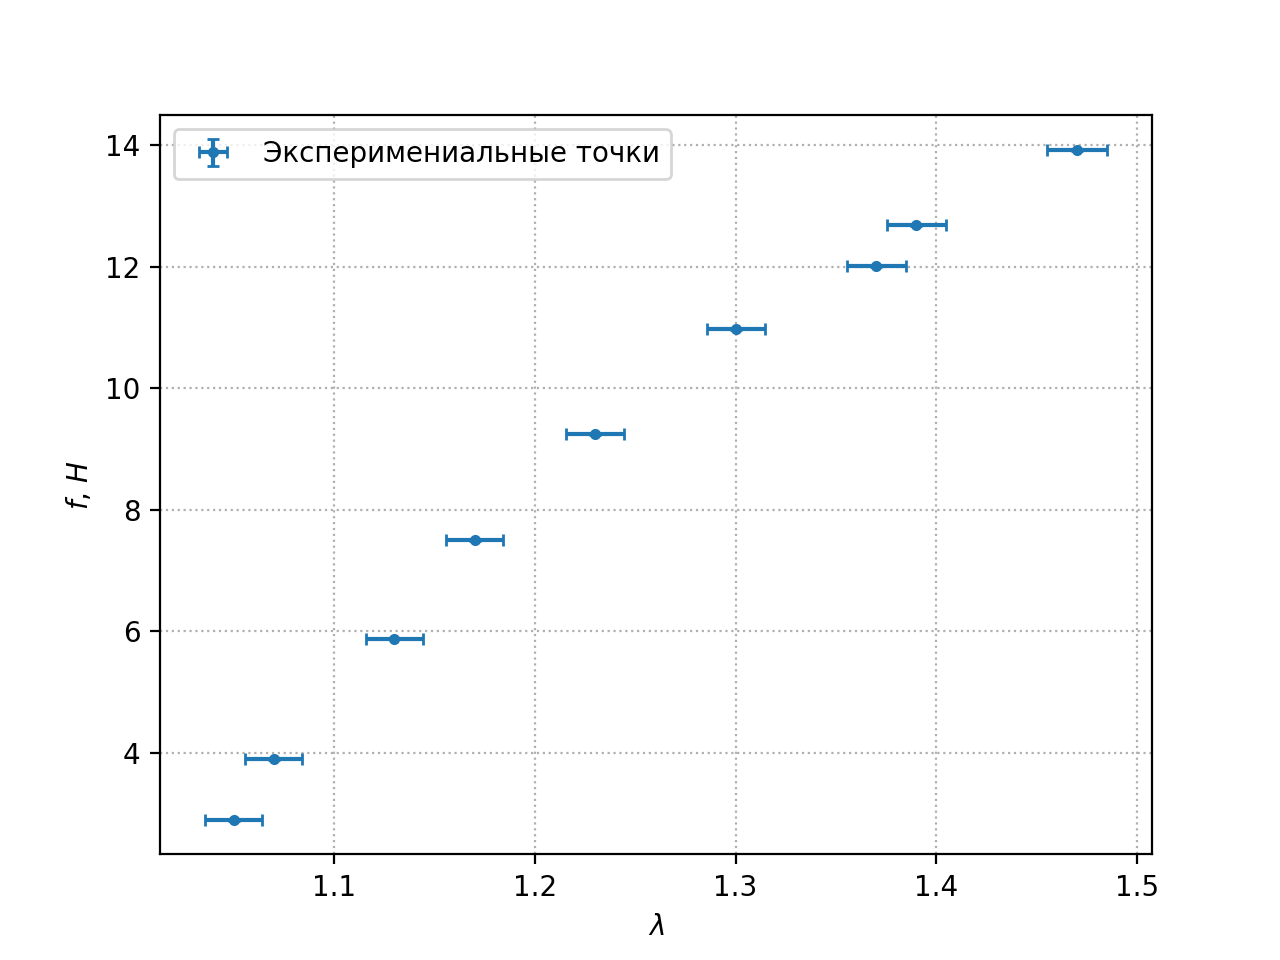
\includegraphics[width=0.89\textwidth]{f(lambda).png}
\caption{$f(\lambda)$ при постоянной температуре.}
\end{center}
\end{figure}

\begin{figure}[h!]
\begin{center}
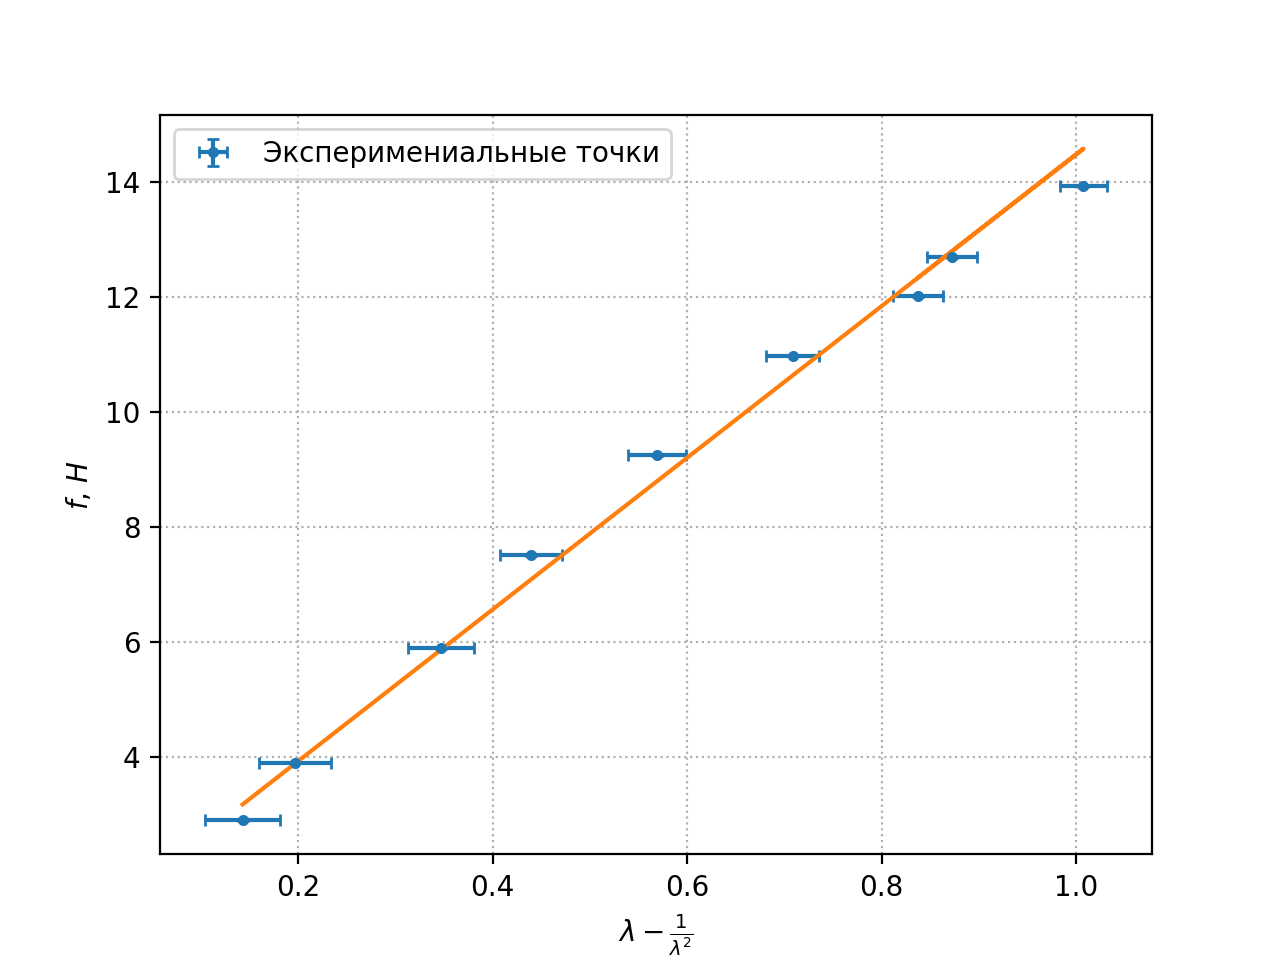
\includegraphics[width=0.89\textwidth]{f(lambda2).png}
\caption{$f(\lambda - \frac{1}{\lambda^2})$ при постоянной температуре.}
\end{center}
\end{figure}

\FloatBarrier

\subsection*{Модуль Юнга}

\begin{equation}\label{young}
    E = (1.33 \pm 0.18) \ МПа
\end{equation}

\subsection*{Работа силы в зависимости от растяжения}

$$A(\lambda) = \frac{1}{3}s_0E(\frac{\lambda^2}{2}+\frac{1}{\lambda}-\frac{3}{2})$$

\begin{figure}[h!]
\begin{center}
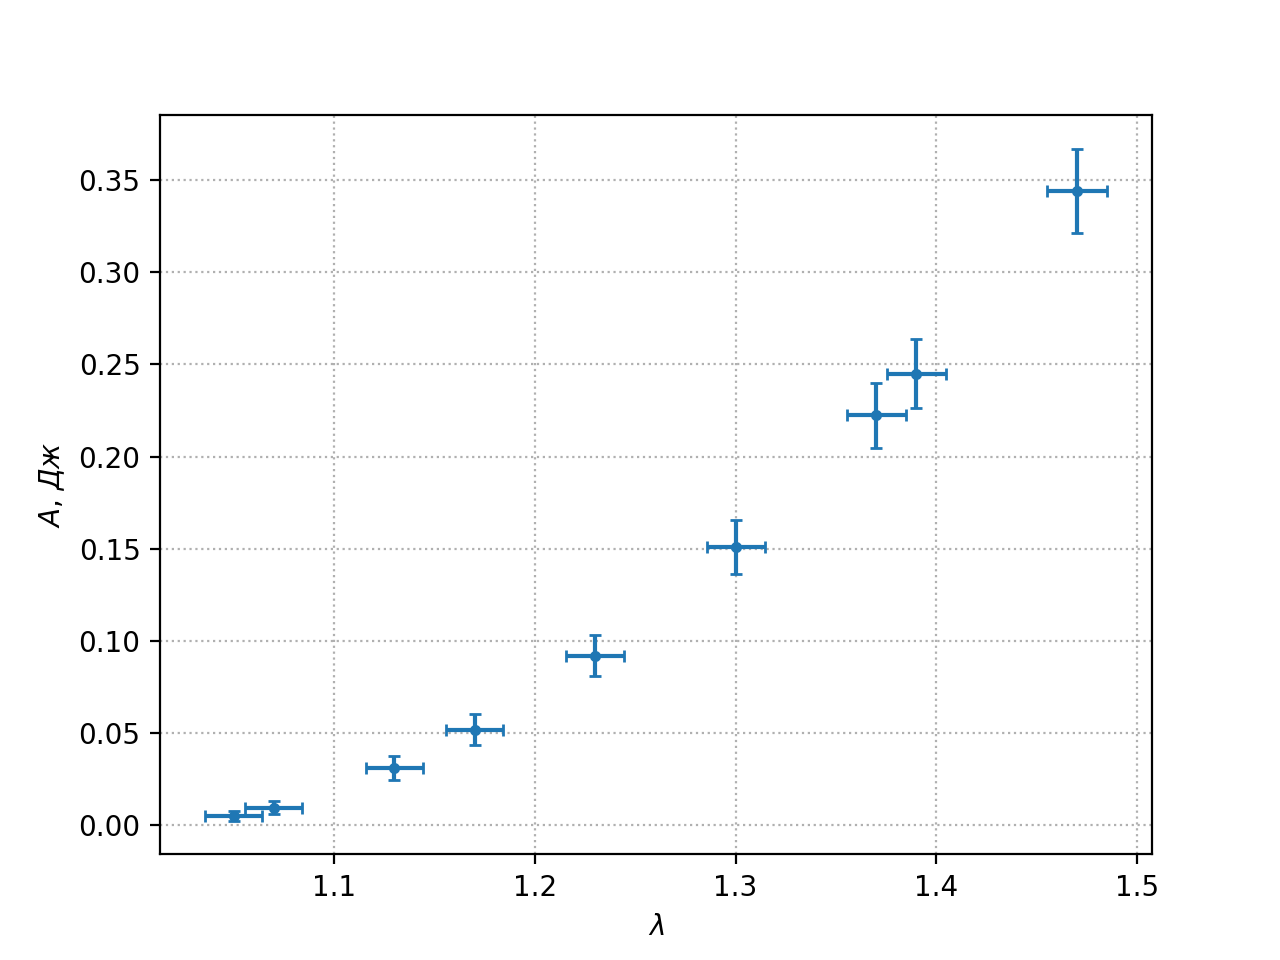
\includegraphics[width=0.57\textwidth]{A(lambda).png}
\caption{$A(\lambda)$ при постоянной температуре.}\label{work}
\end{center}
\end{figure}

\FloatBarrier

\subsection*{Термический эффект при адиабатическом расширении}

\begin{table}[h!]
\begin{tabular}{rrrr}
\toprule
$\Delta t$, $c$ & $N$ & $\Delta P$, $Па$ & $Q$, $мл/с$ \\
\midrule
9.6 & 101 & 196.3 & 104.2 \\
9.1 & 120 & 233.2 & 109.9 \\
8.5 & 154 & 299.3 & 117.6 \\
8.0 & 171 & 332.4 & 125.0 \\
7.8 & 186 & 361.5 & 128.2 \\
7.4 & 206 & 400.4 & 135.1 \\
6.7 & 247 & 480.1 & 149.3 \\
6.2 & 277 & 538.4 & 161.3 \\
\bottomrule
\end{tabular}

\caption{$T(\lambda)$ при адиабатическом расширении.}
\end{table}

\subsection*{Теплоёмкость резиновой полосы}

\begin{figure}[h!]
\begin{center}
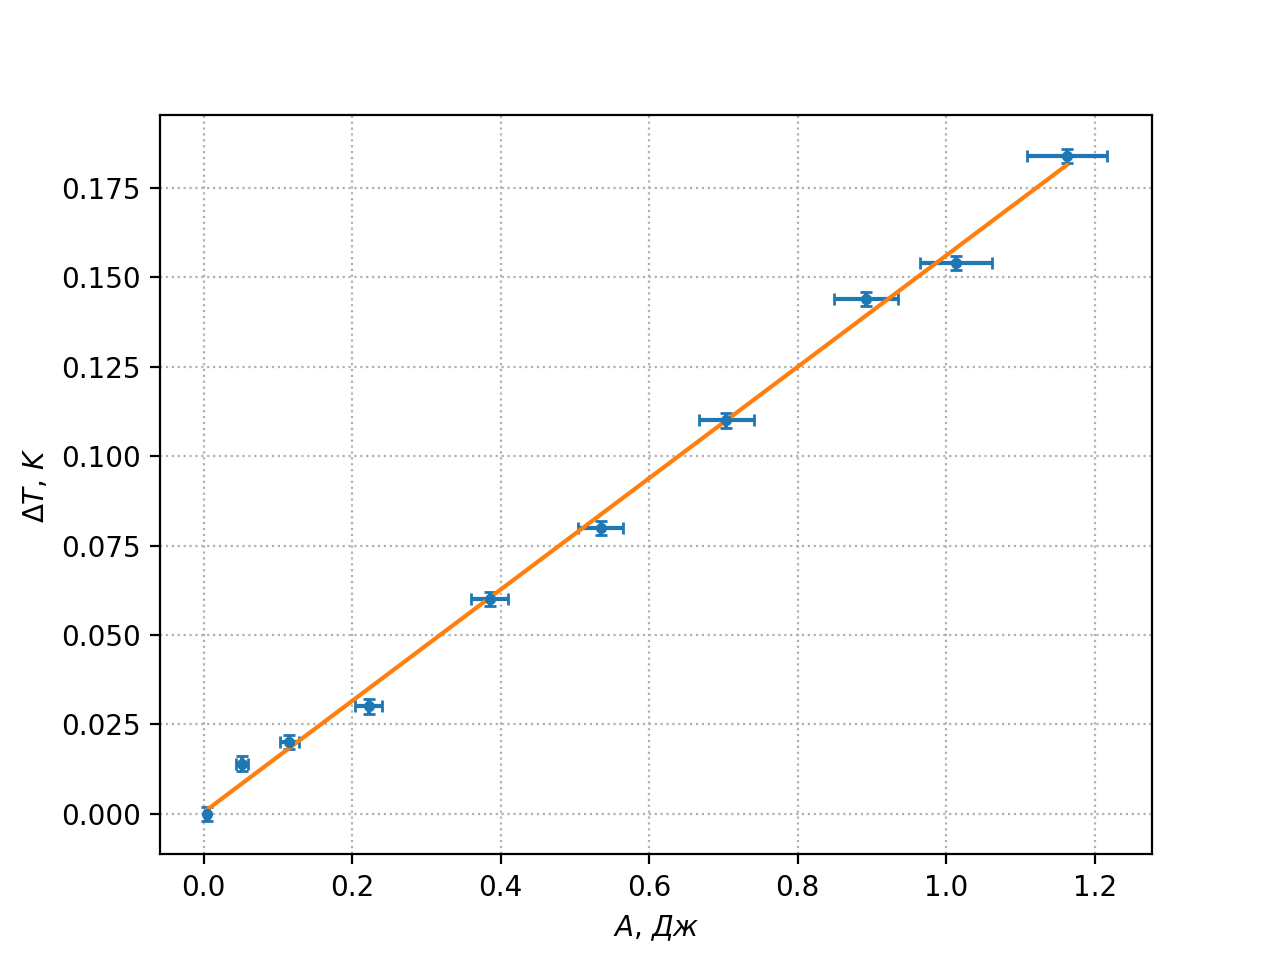
\includegraphics[width=0.89\textwidth]{T(A).png}
\caption{$\Delta T(A)$.}\label{TA}
\end{center}
\end{figure}

\begin{equation}\label{c1}
    C_l = (6.42 \pm 0.13) \ \frac{Дж}{К}
\end{equation}

\begin{equation}\label{c2}
    c_l = (2.23 \pm 0.30) \ \frac{Дж}{г \cdot К}
\end{equation}

\FloatBarrier

\subsection*{Зависимость логарифма приращения температуры от времени}

\begin{figure}[h!]
\begin{center}
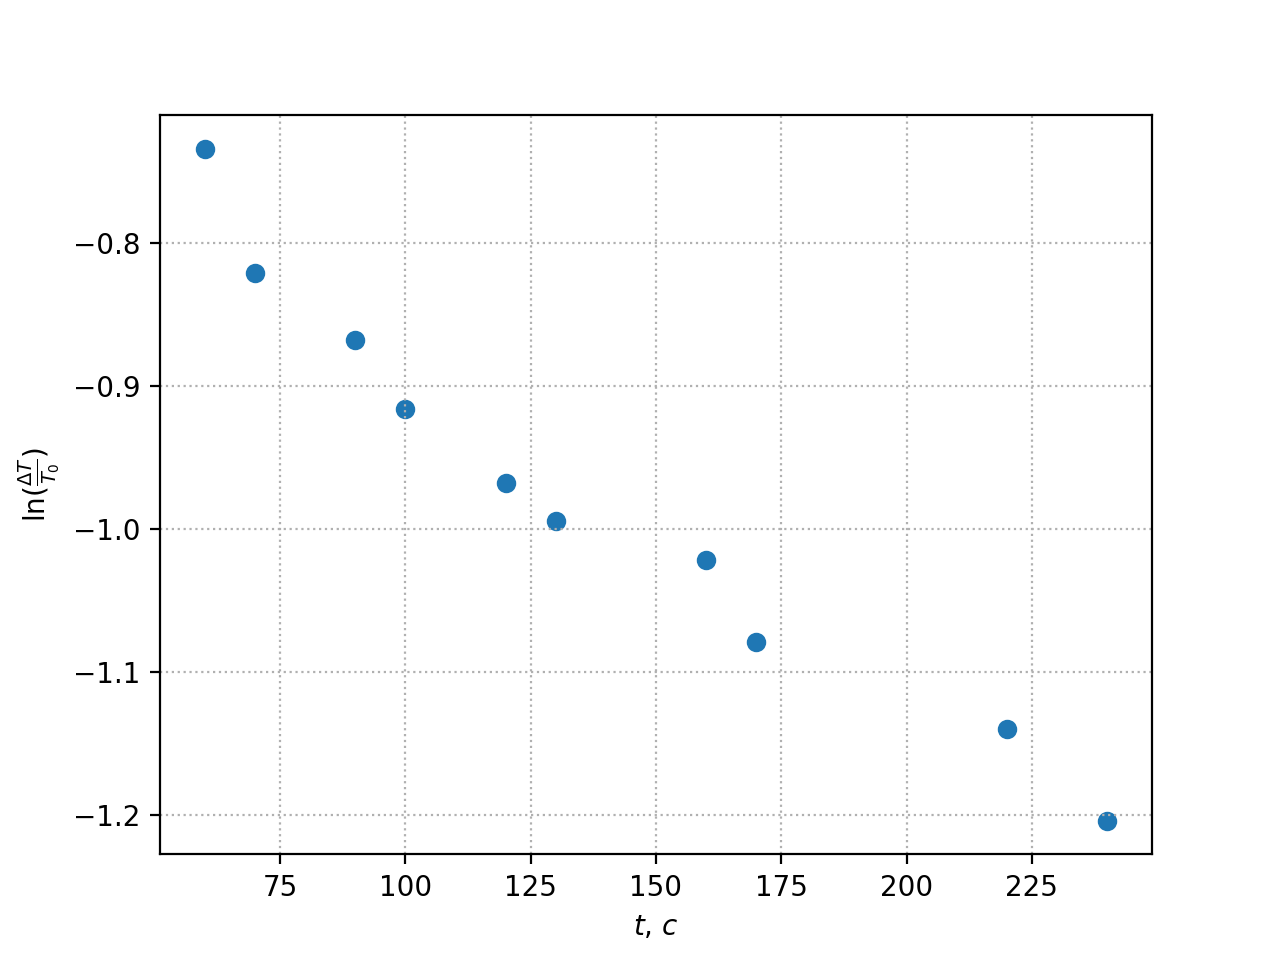
\includegraphics[width=0.89\textwidth]{T(t).png}
\caption{$\ln(\frac{\Delta T}{T_0})(t)$.}\label{Tt}
\end{center}
\end{figure}

\FloatBarrier

\section{Обсуждение результатов}

Зависимость $f(\lambda - \frac{1}{\lambda^2})$ при постоянной температуре является линейной. Все точки легли на прямую в рамках погрешностей за исключением, быть может, одной. Можно считать, что наша модель подчиняется закону Гука.

Вычислен модуль Юнга (\ref{young}).

Теоретически определена зависимость работы силы в зависимости от растяжения рис. (\ref{work}).

По коэффициенту наклона графика зависимости температуры от работы (рис. \ref{TA}) рассчитаны теплоемкости (\ref{c1}) и (\ref{c2}), которые хорошо соотносятся с табличными.

Подтверждена экспоненциальная зависимости температуры от времени (рис. \ref{Tt}).

\end{document}